\documentclass[tikz,border=12pt]{standalone}
\begin{document}
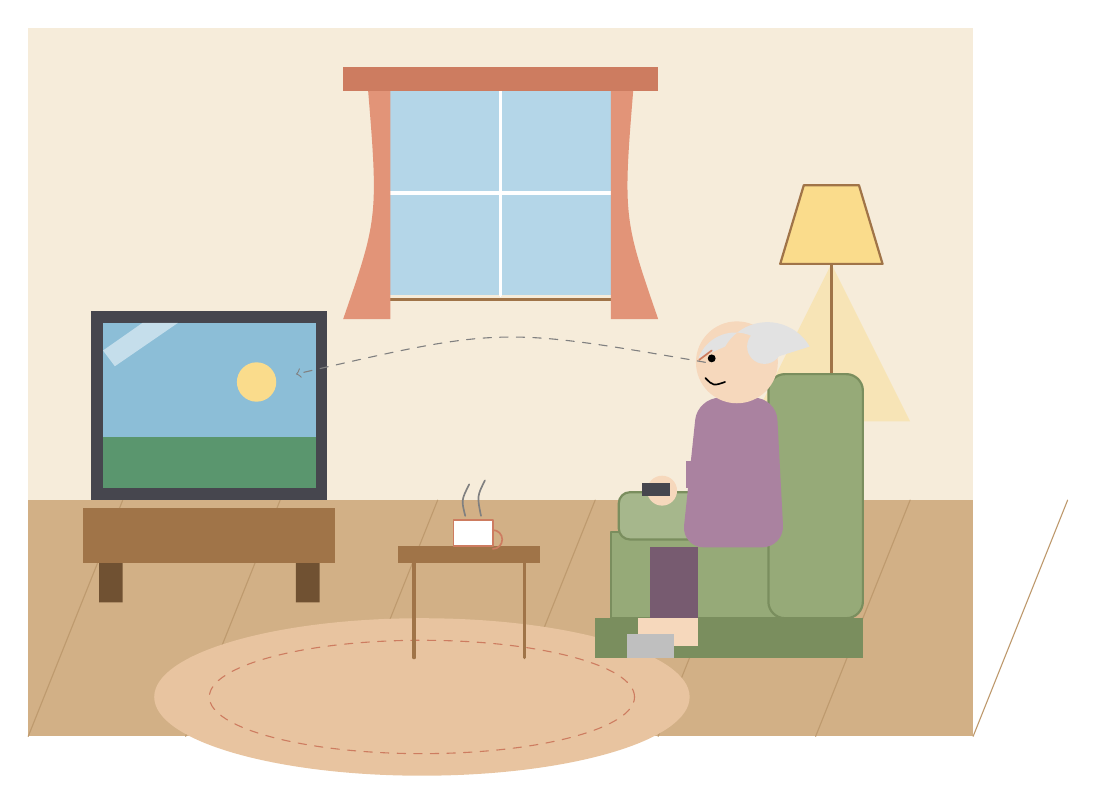
\begin{tikzpicture}[line cap=round,line join=round,scale=1.0]
  \definecolor{wall}{RGB}{246,236,218}
  \definecolor{floor}{RGB}{210,176,134}
  \definecolor{floorline}{RGB}{190,154,110}
  \definecolor{curtain}{RGB}{226,148,120}
  \definecolor{curtaindark}{RGB}{205,124,96}
  \definecolor{windowsky}{RGB}{180,214,232}
  \definecolor{tvframe}{RGB}{70,70,78}
  \definecolor{tvscreen}{RGB}{140,190,215}
  \definecolor{sofa}{RGB}{150,170,120}
  \definecolor{sofadark}{RGB}{122,142,94}
  \definecolor{skin}{RGB}{246,216,188}
  \definecolor{hair}{RGB}{226,226,226}
  \definecolor{dress}{RGB}{170,130,160}
  \definecolor{wood}{RGB}{160,116,72}
  \definecolor{rug}{RGB}{232,196,160}
  \definecolor{lamp}{RGB}{250,220,140}
  \definecolor{tvgreen}{RGB}{90,150,110}

  % room
  \fill[wall] (0,3) rectangle (12,9);
  \fill[floor] (0,0) rectangle (12,3);
  \foreach \x in {0,2,...,12} { \draw[floorline] (\x,0) -- (\x+1.2,3); }

  % window with curtains (back wall, center-left)
  \fill[windowsky] (4.6,5.6) rectangle (7.4,8.2);
  \draw[white,very thick] (6,5.6) -- (6,8.2) (4.6,6.9) -- (7.4,6.9);
  \draw[wood,very thick] (4.55,5.55) rectangle (7.45,8.25);
  \fill[curtain] (4.0,5.3) .. controls (4.45,6.6) .. (4.3,8.4) -- (4.6,8.4) -- (4.6,5.3) -- cycle;
  \fill[curtain] (8.0,5.3) .. controls (7.55,6.6) .. (7.7,8.4) -- (7.4,8.4) -- (7.4,5.3) -- cycle;
  \fill[curtaindark] (4.0,8.2) rectangle (8.0,8.5);

  % floor lamp (right side, warm light)
  \fill[lamp,opacity=0.45] (10.2,6.0) -- (9.2,4.0) -- (11.2,4.0) -- cycle;
  \draw[wood,very thick] (10.2,3.0) -- (10.2,6.0);
  \fill[wood] (9.8,2.9) rectangle (10.6,3.05);
  \fill[lamp,draw=wood,thick] (9.55,6.0) -- (10.85,6.0) -- (10.55,7.0) -- (9.85,7.0) -- cycle;

  % TV on wooden stand (left side)
  \fill[wood] (0.7,2.2) rectangle (3.9,2.9);
  \fill[wood!70!black] (0.9,1.7) rectangle (1.2,2.2) (3.4,1.7) rectangle (3.7,2.2);
  \fill[tvframe] (0.8,3.0) rectangle (3.8,5.4);
  \fill[tvscreen] (0.95,3.15) rectangle (3.65,5.25);
  \fill[white,opacity=0.5] (1.1,4.7) -- (1.9,5.25) -- (1.45,5.25) -- (0.95,4.9) -- cycle;
  % simple program on screen
  \fill[tvgreen] (0.95,3.15) rectangle (3.65,3.8);
  \fill[lamp] (2.9,4.5) circle (0.25);

  % rug
  \fill[rug] (5.0,0.5) ellipse (3.4 and 1.0);
  \draw[curtaindark,dashed] (5.0,0.5) ellipse (2.7 and 0.72);

  % small table with teacup
  \fill[wood] (4.7,2.2) rectangle (6.5,2.42);
  \draw[wood,very thick] (4.9,1.0) -- (4.9,2.2) (6.3,1.0) -- (6.3,2.2);
  \fill[white,draw=curtaindark,semithick] (5.4,2.42) rectangle (5.9,2.75);
  \draw[curtaindark,semithick] (5.9,2.62) arc[start angle=90,end angle=-90,radius=0.12];
  \draw[gray,semithick] (5.55,2.8) .. controls (5.5,3.0) .. (5.6,3.2);
  \draw[gray,semithick] (5.75,2.8) .. controls (5.7,3.05) .. (5.8,3.25);

  % sofa (right, facing left toward TV)
  \fill[sofadark] (7.2,1.0) rectangle (10.6,1.5);
  \fill[sofa,draw=sofadark,thick] (7.4,1.5) rectangle (10.4,2.6);
  \fill[sofa,draw=sofadark,thick,rounded corners=6pt] (9.4,1.5) rectangle (10.6,4.6);
  \fill[sofa!85!white,draw=sofadark,thick,rounded corners=4pt] (7.5,2.5) rectangle (9.3,3.1);

  % grandma sitting on sofa, facing left (toward TV)
  % legs
  \fill[dress!70!black] (7.9,1.5) rectangle (8.5,2.4);
  \fill[skin] (7.75,1.15) rectangle (8.5,1.5);
  \fill[gray!50!white] (7.6,1.0) rectangle (8.2,1.3);
  % body
  \fill[dress,rounded corners=8pt] (8.3,2.4) -- (9.6,2.4) -- (9.5,4.3) -- (8.5,4.3) -- cycle;
  % arm holding remote toward TV
  \fill[dress] (8.35,3.15) rectangle (9.2,3.5);
  \fill[skin] (8.05,3.12) circle (0.19);
  \fill[tvframe] (7.8,3.05) rectangle (8.15,3.22);
  % head facing left
  \fill[skin] (9.0,4.75) circle (0.52);
  \fill[hair] (8.85,4.95) arc[start angle=150,end angle=30,radius=0.62] -- (9.45,4.8) arc[start angle=20,end angle=160,radius=0.5] -- cycle;
  \fill[hair] (9.35,4.95) circle (0.22);
  % face details: eye looking left, smile
  \fill[black] (8.68,4.8) circle (0.05);
  \draw[black,semithick] (8.6,4.55) .. controls (8.7,4.45) .. (8.85,4.5);
  \draw[curtaindark,semithick] (8.52,4.78) -- (8.68,4.9);

  % gaze line from grandma to TV
  \draw[gray,dashed,->] (8.6,4.75) .. controls (6.0,5.2) .. (3.4,4.6);
\end{tikzpicture}
\end{document}
